
\documentclass[11pt]{article}
\usepackage{graphicx}
\begin{document}

\section{
Howto Guide to Tunnel Junction Noise Metrology}

<h4> I. Fabrication </h4>




This guide mostly assumes you already have a good tunnel junction, since it is a somewhat involved process to get good fab working from scratch. By far the easiest and most reliable way to get a good device is to have Joe Aumentado at NIST send you one.  Given the resources for fab available at NIST, Joe's experience with the fab, and the small number of people who will ever want or need these devices, this is a good system for supply for the time being.  Should Joe ever retire from NIST this capability will hopefully be passed on to future NIST staff, or if not to other national metrology lab staff in another country, since it is effectively a reference material even if it's not yet classified as such.    




    Future generations of this document will eventually have full fabrication details and get merged with internal NIST documentation to make a coherent information structure but for now, a pointer to Joe's lab at NIST is the best option.


<h4>II. Installation in Fridge</h4>



In order to get this device in the fridge you first need to put the chip in an appropriate sample box.  Again the most reliable way to get this right the first time is to get a device directly from Joe Aumentado at NIST and use his design of sample box and board.  Typically what is used is an OFHC machined copper box with one SMA port which launches to a circuit board designed to match silicon wafers in both thickness and dielectric constant(about 300 microns and 10-11, raspectively).  This box has a cavity machined in it with the size for a rare earth magnet to sit which will keep the aluminum normal.  If you're using this in a experiment with qubits this can be problematic since you don't want stray fields to affect your other experiments.  There is no well established way to solve this problem at this time.  Junctions can be fabricated with manganese doped aluminum which don't require a magnetic field to remain normal at all temperatures, and if this were ever scaled up that is the correct solution.  In the mean time if you have a large magnet on your fridge you can ramp that up for this experiment then ramp it back down for your qubit experiments, or put the tunnel junction as far as you can from the qubits, and add mu metal shielding as needed.




    The next stage after the sample holder is the bias tee.  The bias tees which are widely trusted cold over large frequency range are the Anritsu bias tees, which go up to almost 20 GHz.

<h4>III. Pre-Cooldown and Cooldown Checklist</h4>

\begin{figure}

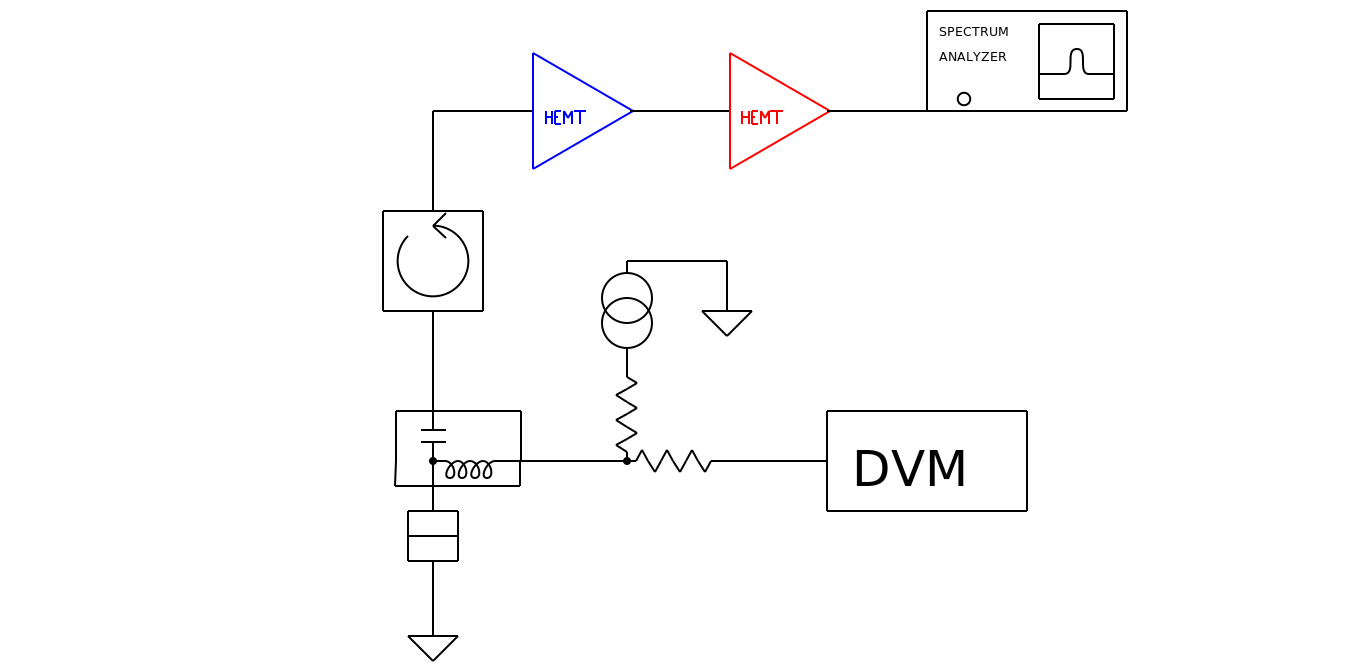
\includegraphics[width=\linewidth]{../svg/svg1519861628.svg}

\caption{Figure x. }
\end{figure}


<ol>
    <li>
        Test that your method of doing an IV curve works on a resistor first.  To do this, put a 50 ohm resistor(or 100 ohm if that's more convenient, but it should be near 50) and put it in the fridge, warm, exactly where the shot noise device will go.  To do this you need two DC lines connecting to the DC side of your bias tee, and they should both have bias resistors which can go cold.  Now sweep the voltage on one of the two DC lines and measure the voltage on the other.  You should be able to calculate a resistance which makes sense based on knowing your bias resistors.  Also important here is to establish that your bias scheme will keep the voltage on the device to at or below about 100 mV so that you know you won't blow the device, which happens somewhere between 100 mV and 500 mV generally, but 100 mV is a good solid safety margin.  Generally what you want is to have the triangle wave output of your audio function generator be several volts peak to peak but with enough voltage division so that even at the maximum voltage you are safe or at least close to the safe zone.
    </li>
    <li>
        After you know you can trust your IV curve bias system, power down the system, short anything to ground that you can, and connect the dc line back to your tunnel junction device.  Now ramp up the voltage on your bias system and see the IV curve on the oscilloscope and check that you get a value that makes sense.  The NIST devices are generally pretty close to 50 Ohms, where "pretty close" is usually in the 10% range or better.  Resistances change a few percent on cooling so don't worry about being closer than that.  You want to be able to convince yourself that the resistance is between 40 and 60 Ohms at this stage.  20-100 works, but again if you're using NIST devices that is outside what you expect because those are pretty accurate to the 50 Ohm target.
    </li>
    <li>
        When you're sure you have a live device, you want to test your RF chain.  Start by computing the total gain in the chain, including all HEMTs.  With a 40 dB cold HEMT and another 20-40 dB of warm gain, a 4 K input noise should translate to at least hundreds of thousands of kelvin at the output, which is enough to get over the noise floor of your spectrum analyzer.  If this is a new setup, test the full chain with a network analzyer, putting enough attenuation on the input to make sure you don't saturate the amps.  If you put attenuation equal to estimated gain, the whole thing should have insertion loss around 0 dB and you should not have problems doing a simple network analyzer measurement.  Check that this makes sense, then disconnect the network analyzer, put the junction back in, and check the spectrum analzyer as you power the amps down and back up and see that the noise level on the spectrum analzyer rises and falls as you expect.  This is again just a sanity check and does not have to be accurate(it won't be).  You want, qualitatively, to see that the noise rises enough to swamp existing noise level as you first power up the warm amp, then the cold amp.  When you're sure the RF noise makes sense and RF insertion loss of the whole system makes sense, make sure the shot noise junction is connected.
    </li>
    <li>
        Test that the shot noise device can boost noise warm.  Now you put together the above tests, and power up both "cold" and warm amps, then increase the bias on the junction to 100 mV and see that this shifts the noise in a noticeable way.  With room temprature kT/e being about 25 mV this is about 4 kT/e, so it should be clearly visible, although if you look at a curve of the noise at this point it is mostly parabolic and won't be useful for metrology yet. 
    </li>
    <li>
        If you know your device makes shot noise that you can measure, it's time to connect the system to take shot noise curves.  This means sweeping your IV curve and simultaneously looking at the spectrum analyzer in zero span mode, triggered off of he sweeper that is driving the IV curve using the external trigger of the spectrum analzyer.  This is the measurement you will do cold, but warm.  You should see a sequence of parabolas on the spectrum analyzer.  Once this all works, you can power off the sweeper and amps for the inital cooldown.
    </li>
    <li>
        Now that you know you have a working RF chain, working DC bias system, and working combined RF/DC with a shot noise curve, you can cool your fridge to whatever the first obvious test point is, probably before you start circulating mix.  At that point, you want to lower the bias sweep voltage and try the full test again.  A rule of thumb is that you want about 10 kT/e on the device.  So if you're at 30 kelvin that's 10 times 2.5 mV is 25 mV maximum voltage.  At 3 kelvin you sweep to plus and minus 2.5 mV, and so on down to base where you'll be sweeping at a fraction of a mV.  
    </li>
    <li>
        Now that you're cold and have a working shot noise device with a noise-voltage curve that makes sense, you want to start acquiring and analyzing data.  To do this, figure out how to get a sweep out of your spectrum analyzer over GPIB or ethernet, and get a reliable value for the sweep amplitude in real volts on the device using your volt meter or a oscilloscope or daq card.
    </li>
</ol>

<h4>Numerical Details of Measurement</h4>

$$
P = T_N \ + \frac{1}{2}T\left[\frac{V+F}{2T}\coth{\frac{V+F}{2T}}
+ \frac{V-F}{2T}\coth{\frac{V-F}{2T}}\right]
$$
In this formula everything is in units of pixels on the screen in the plot on the computer.  Gains specific to the 

$$
E = h\nu
$$
<h4>IV. What went wrong?</h4>

<ul>
<li>No RF connectivity</li>
<li>No DC connectivity</li>
<li>RF connected, but noise temperature much higher(10x or more) than it should be</li>
<li>Dead junction(generally short)</li>
<li>Everything seems to work but noise temperature is a bit (1.5-5x) higher than you hoped/expected.</li>
<li></li>
<li></li>

</ul>

<h4>V. Analyze your Data</h4>

<h4>VI. Amplifier Metrology</h4>

<h4>VII. Future Work</h4>
\end{document}
